% -*- root: ../Presentation.tex -*-
\section{Forbedringer}
\begin{frame}{Forbedringer til programmet}{}
	Problemer vi ville løse:
	\begin{itemize}
		\item Primitiv tilgang til \lstinline|Graph| klassens opbygning
		\item Megen funktionalitet gemt i \lstinline|JPEGImage| klassen
	\end{itemize}
\end{frame}

\subsection{Ændringer til \lstinline|Graph|}
\begin{frame}{Ændringer til \lstinline|Graph|}{}
	3 forskellige måder at opbygge en graf:
	\begin{enumerate}
		\item Liste af Vertices og Edges\uncover<2-2>{\textcolor{red}{$\leftarrow$}}
		\item Naboliste (Adjacency List)\uncover<3-3>{\textcolor{red}{$\leftarrow$}}
		\item Nabomatrix (Adjacency Matrix)
	\end{enumerate}
\note<.-> {
	I afsnit 3.3  diskuteres forskellige fremstillinger. Vi bruger den simple, men beskriver adjancency listen som værende en god ide.

	Vi havde et ønske om at benytte den
}
\end{frame}

\begin{frame}{Fordel ved naboliste}{}
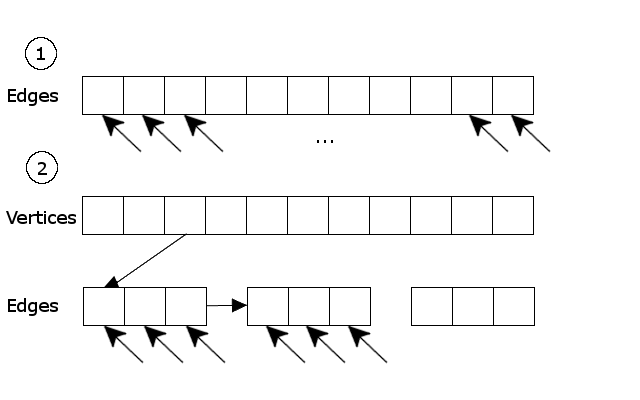
\includegraphics[width=\textwidth]{figures/graphLists.png}
\note<.-> {
	(1)
	For at slette en kant skal vi loope igennem alle vores kanter, og kun slette dem vi skal bruge.
	Resulterer i mange spildte operationer

	(2)
	Vi skal kun loope igennem de kanter der bliver peget på af edges i naboerne til en vertex
}
\end{frame}



\begin{frame}[fragile]{Svaret er...}{}
\lstinline|GraphEncoder|
\begin{itemize}
	\item Håndterer alt graf-enkodning
	\item En generel løsning fremfor specialsyet til JPEG
	\item Maksimerer data-hiding og testabilitet
\end{itemize}

\only<1-1> {
	\lstinputlisting[breaklines=true,basicstyle=\tiny,frame=single]{Mathias/code1.cs}
}
\only<2-2> {
	\lstinputlisting[breaklines=true,basicstyle=\tiny,frame=single]{Mathias/code2.cs}
}
\note<.->{
	Vi kan gemme alt graf væk fra JPEG. Det er kun grafen selv der behøver at kende til det.

	Dette betyder at løsningen kan fungere på ``alle'' tal. Ikke kun AC koefficienter. GraphEncoder er ligeglad hvor tallene kommer fra

	Vi kan gøre løsningen mere fleksibel ved hjælp af interfaces

	Forskellige typer af graffremstillinger kunne skiftes ud på runtime eller når et nyt bliver lavet
}
\end{frame}